\documentclass{beamer}
%\documentclass[handout]{beamer}

% Input all common stuff


% THEME SETTINGS %%%%%%%%%%%%
\usetheme[secheader]{Boadilla}
\usecolortheme{default}
\useinnertheme{circles}
\setbeamertemplate{blocks}[default]

% Get rid of bottom navigation bars
\setbeamertemplate{footline}[page number]{}

% Gets rid of navigation symbols
\setbeamertemplate{navigation symbols}{}

% PACKAGES %%%%%%%%%%%%%%%%%%%
\usepackage{listings}
\usepackage{xcolor}
\usepackage{multirow}
\usepackage{array}
\usepackage{verbatim}
\usepackage{pbox}
\usepackage{tabularx}

% LISTINGS STYLE %%%%%%%%%%%%%
\definecolor{bluekeywords}{rgb}{0.13,0.13,1}
\definecolor{greencomments}{rgb}{0,0.5,0}
\definecolor{redstrings}{rgb}{0.9,0,0}
\definecolor{listingsbg}{HTML}{EFEFFF}

\lstset{language=C++,
  showspaces=false,            % show spaces adding particular underscores
  showtabs=false,              % show tabs within strings adding particular underscores
  breaklines=true,             % sets automatic line breaking
  showstringspaces=false,      % underline spaces within strings
  breakatwhitespace=true,      % sets if automatic breaks should only happen at whitespace
  captionpos=b,                % sets the caption-position to bottom
  escapeinside={(*@}{@*)},
  commentstyle=\color{greencomments},
  keywordstyle=\color{bluekeywords}\bfseries,
  stringstyle=\color{redstrings},
  basicstyle=\ttfamily\fontsize{9}{10}\selectfont,
  backgroundcolor=\color{listingsbg}
}

% MACROS %%%%%%%%%%%%%%%%%%%%%
\newcommand{\lstsrctitle}[0]{%
 {\scriptsize\lstname}
}

\newcommand{\kw}[1]{\texttt{\textcolor{bluekeywords}{\ttfamily\fontsize{9}{10}\selectfont #1}}}

\newenvironment{varblock}[3]{%
  \setbeamercolor{block body}{#2}
  \setbeamercolor{block title}{#3}
  \begin{block}{#1}}{\end{block}}

% Colours taken from http://twitter.github.com/bootstrap/components.html#alerts
% Do block %%%%%%%%%%%%%%%%%%%%%%
\definecolor{doblocktext}{HTML}{468847}
\definecolor{doblockbg}{HTML}{DFF0D8}
\newenvironment{doblocke}[0]{% begin
  \begin{varblock}{\textbf{Do}}%
  {bg=doblockbg,fg=doblocktext}{bg=doblocktext,fg=white}%
  \setbeamercolor{itemize item}{fg=doblocktext}
  \lstset{backgroundcolor=}% The background should be the same as that of the block
  } % begin
  {\end{varblock}} %end
  
\newcommand{\doblock}[1]{%
 \begin{doblocke}#1\end{doblocke} 
}

% Don't block %%%%%%%%%%%%%%%%%%%
\definecolor{dontblocktext}{HTML}{B94A48}
\definecolor{dontblockbg}{HTML}{F2DEDE}  
\newenvironment{dontblocke}[0]{% begin
  \begin{varblock}{\textbf{Don't}}%
  {bg=dontblockbg,fg=dontblocktext}{bg=dontblocktext,fg=white}
  \setbeamercolor{itemize item}{fg=dontblocktext}
  \lstset{backgroundcolor=}% The background should be the same as that of the block
  }%
  {\end{varblock}} %end

\newcommand{\dontblock}[1]{%
 \begin{dontblocke}#1\end{dontblocke} 
}

% Defi block %%%%%%%%%%%%%%%%%%%%
\definecolor{defiblocktext}{HTML}{3A87AD}
\definecolor{defiblockbg}{HTML}{D9EDF7}
\newenvironment{defiblocke}[1]{% begin
  \begin{varblock}{\textbf{Definition}}%
  {bg=defiblockbg,fg=defiblocktext}{bg=defiblocktext,fg=white}
  \lstset{backgroundcolor=}% The background should be the same as that of the block
  \textit{#1} }
  {\end{varblock}} %end

\newcommand{\defiblock}[2]{%
 \begin{varblock}{\textbf{Definition}}%
 {bg=defiblockbg,fg=defiblocktext}{bg=defiblocktext,fg=white}%
  \begin{tabularx}{\linewidth}{lX}\textit{#1} & #2\end{tabularx}
 \end{varblock} 
}

\newenvironment{defiblockbaree}[1]{ %begin
  \begin{varblock}{\textbf{#1}}%
  {bg=defiblockbg,fg=defiblocktext}{bg=defiblocktext,fg=white}
  \lstset{backgroundcolor=}} %begin
  {\end{varblock}} %end

\definecolor{warnblocktext}{HTML}{C09853}
\definecolor{warnblockbg}{HTML}{FCF8E3}
\newenvironment{warnblocke}[0]{% begin
  \begin{varblock}{\textbf{Warning!}}%
  {bg=warnblockbg,fg=warnblocktext}{bg=warnblocktext,fg=white}
  \lstset{backgroundcolor=}% The background should be the same as that of the block
  \setbeamercolor{itemize item}{fg=warnblocktext}
  \setbeamercolor{item projected}{fg=white,bg=warnblocktext}
  } % begin
  {\end{varblock}} % end

\newcommand{\warnblock}[1]{%
  \begin{warnblocke}#1\end{warnblocke}
} % newcommand

\newcommand{\cout}[1]{%
 Output: \pbox[t]{\textwidth}{\ttfamily\fontsize{9}{10}\selectfont{}#1}
}

\newenvironment{doitemize}[0]{%
  \begin{itemize}}%
  {\end{itemize}} %end


% CONSTANTS %%%%%%%%%%%%%%%%%%%%%%%%%%%

%Symbol for backslash in texttt \char`\\

% Common title slide stuff
\title{Introduction to Scientific Programming with C++}
\author{Martin Uhrin}
\institute{UCL}
\date{February 11-13th 2013}

\subtitle{Session 0: Basics}

\usepackage{graphicx}

\begin{document}

\frame{\titlepage}

\begin{frame}
\frametitle{Table of Contents}
\tableofcontents
\end{frame}

\section{Introduction to language}

\begin{frame}
	\frametitle{Introduction to C++}
	\framesubtitle{A little history}
	\begin{itemize}
	  \item<1->{Created in 1979 as an extension of C by this guy:\pause
		\begin{figure}
			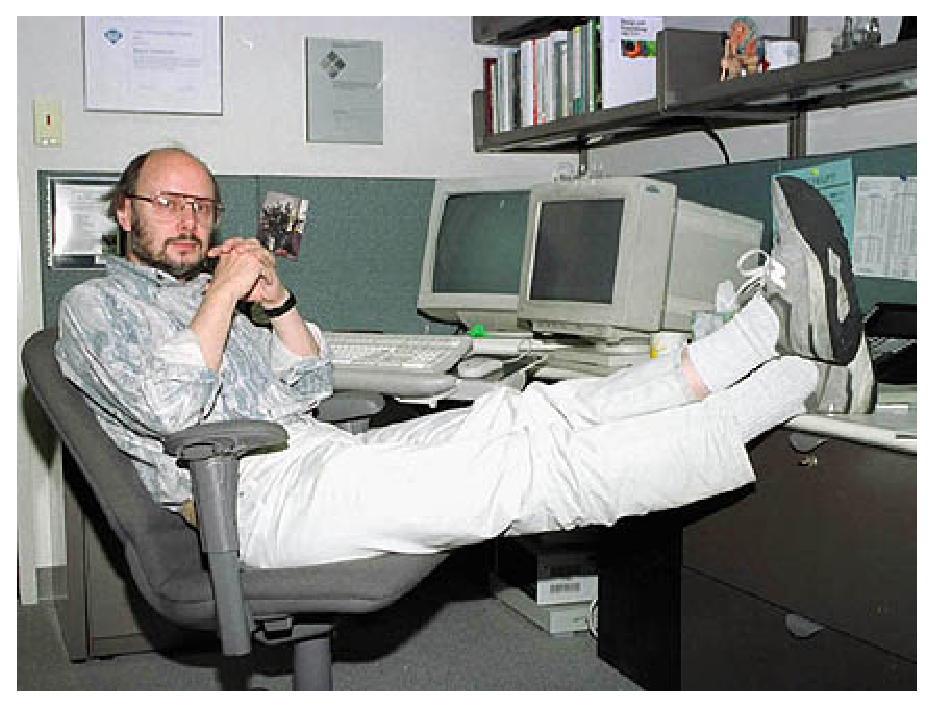
\includegraphics[height=30mm]{./figs/BjarneStroustrup.eps}
			\caption{Bjarne Stroustrup, creator of C++.}
		\end{figure}}
	  \item<3->{Built to be fast \textit{and} scalable and so has a mix of high and low-level constructs.}
	\end{itemize}
	
\end{frame}


\section{Program structure}

%Perhaps the best way to learn a programming language is to dive in and see what it's all about with a simple example.

%Here's out first program:

\begin{frame}[fragile]
  \frametitle{Hello World!}
  \framesubtitle{Where it all begins}

  \begin{columns}[t]
    \begin{column}[T]{0.55\textwidth}	\lstinputlisting[language=C++,title=\lstsrctitle,aboveskip=0pt]{../code/0_basics/lectures/hello_world.cpp}
    \end{column}
    \begin{column}[T]{0.45\textwidth}
			\cout{Hello world!}
		\end{column}
	\end{columns}
\end{frame}


\begin{frame}[fragile]
  \frametitle{Hello World dissection}
  \begin{semiverbatim}
  \uncover<1->{// My first C++ program
  }
  \uncover<2->{#include <iostream>
  }
  \uncover<3->{int main()}
  \uncover<4->{\{}
  \uncover<6->{  std::}\uncover<5->{cout << "Hello World!";}
  \uncover<7->{  return 0;}
  \uncover<4->{\}}
  \end{semiverbatim}
\end{frame}

\begin{frame}
  \frametitle{Going from source code to an executable}
  
  \begin{figure}%
    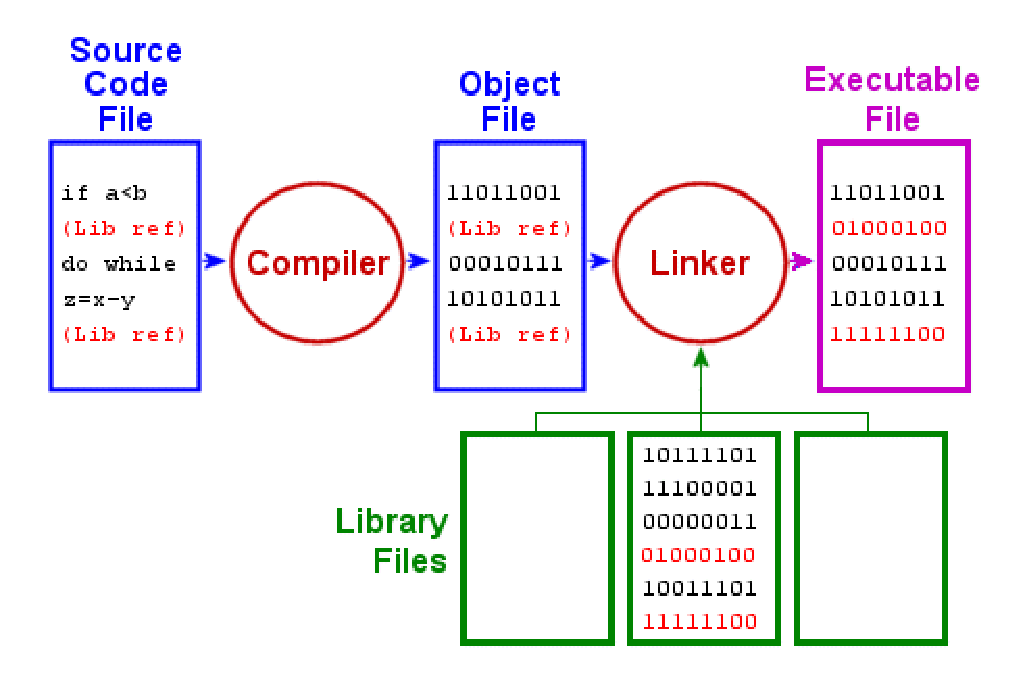
\includegraphics[width=0.6\columnwidth]{figs/compile.eps}%
    \caption{Compilation and linking of a C++ program\footnote{Source \url{http://www.aboutdebian.com/compile.htm} \copyright{} Keith Parkansky}.}%
  \end{figure}
  \pause There are range of compilers, some common ones are \emph{g++} (GNU), \emph{icc} (Intel), \emph{pgicc} (PGI) and others. 

\end{frame}

\begin{frame}[fragile]
  \frametitle{Whitespace}
  \defiblock{whitespace}{spaces, tabs, and (sometimes) new lines.}
  \pause
  
  Completely equivalent as far as compiler is concerned:
  \begin{lstlisting}
#include <iostream>
int main(){std::cout<<"Hello world!";return 0;}
  \end{lstlisting}
  \begin{lstlisting}
#include <iostream>
int main()
{
std::cout
<<
"Hello world!"
;
return
0
;
}  \end{lstlisting}
\end{frame}

\begin{frame}[fragile]
  \frametitle{Case sensitivity}
  C++ is case sensitive!  This means that:
  \begin{lstlisting}
int main()
  \end{lstlisting}
  is different from
  \begin{lstlisting}
INT MAIN ()
  \end{lstlisting}
  which is different from
  \begin{lstlisting}
int Main()
  \end{lstlisting}
  and only the first version is correct.
\end{frame}

\begin{frame}[fragile]
  \frametitle{Comments}
  Two types of comment can be used:
  \begin{lstlisting}
// This is a line comment.
// It ends at the end of the line.
// int myVariable = 0; This code will not execute!
  \end{lstlisting}
  \begin{lstlisting}
/* This is a C-style comment.
   It ends when the closing star-slash is reached. */
  \end{lstlisting}
    Use comments liberally - they are enormously useful!
    \doblock{Avoid stating the obvious.  A good comment will not say \textit{what} is happening but rather \textit{why}.}
\end{frame}

\section{Variables, constants and data types}

\subsection{Defining variables}

\begin{frame}[fragile]
\frametitle{Defining a variable}
  \defiblock{variable}{A named portion of memory used to store a determined value.}
  Let's define some variables:
  \begin{lstlisting}
int anInteger;
double aDouble;
unsigned short i;
float x, y, z;
  \end{lstlisting}
Format: \texttt{\textcolor{bluekeywords}{variable\_type} variable\_name, variable\_name2;}

\end{frame}

\subsection{Naming variables}

\begin{frame}
  \frametitle{Naming variables}
  
  A variable name is an example of an identifier.
  \defiblock{identifier}{an identifier is a sequence of characters used to denote the name of a variable, function\footnote{We'll see what these are shortly.}, class\footnotemark[\value{footnote}] or any entity you need to refer to in your code.}
  \pause
  Identifiers can be any sequence of letters, digits or underscore characters but they must \emph{not}:
	\begin{itemize}
  	\item start with a digit,
	  \item be one of the reserved keywords\footnote{See \url{http://en.cppreference.com/w/cpp/keyword} for full list.}.
	\end{itemize}
	\pause
	\defiblock{keyword}{a word that has a special meaning in the C++ language.}
\end{frame}

\begin{frame}[fragile]
  \frametitle{Naming variables}
  \begin{doblocke}
    \begin{doitemize}
      \item{
			Give variables meaningful names, even if this means more typing!\newline
			Good: \texttt{daysOfWeek, sumSq, isEnabled, unitCell}\newline
			Would the variable name make sense in that context when looking at the code a year later?
			}
			\pause
		  \item{Use variable names, much like comment, to convey intent, e.g.:
		  \begin{lstlisting}
		  double rootMeanSquare; // .. go on to calculate rms
		  \end{lstlisting}}
		  This will make it obvious to the user that the code after this variable should calculate the rms and store it in this variable.
		\end{doitemize}
	\end{doblocke}
	\pause
	\begin{dontblocke}
	  Use abbreviations unless they're VERY common.\newline
	  Use bad names: \texttt{data, dRange, a, ccn, value, one}
	\end{dontblocke}
\end{frame}

\begin{frame}[fragile]
  \frametitle{Variable types}
  Fundamental data types:

% Make the table less cramped vertically. 
% Make sure to reset to 1 after the table!
\renewcommand{\arraystretch}{1.1}
\begin{tabular}{lll}
\hline
Type & Size & Values \\
\hline
\kw{bool} & 1 byte & true or false \\
\kw{int} & 4 bytes & -2,147,483,648 to 2,147,483,647 \\
\kw{double} & 8 bytes & 2.2e-308 to 1.8e308\\ \pause
\kw{char} & 1 byte & 256 character values \\
\kw{unsigned short int} & 2 bytes & 0 to 65,353 \\
\kw{short int} & 2 bytes & -32,768 to 32,767 \\
\kw{unsigned int} & 4 bytes & 0 to 4,294,967,295 \\
\kw{unsigned long int} & 8 bytes & 0 to 18,446,744,073,709,551,615 \\
\kw{long int} & 8 bytes & -9,223,372,036,854,775,807 to \\
 & & 9,223,372,036,854,775,807 \\
\kw{float} & 4 bytes & 1.2e-38 to 3.4e38 
\end{tabular}
\end{frame}
\renewcommand{\arraystretch}{1}

\begin{frame}[fragile]
 \frametitle{Using variables}
 \lstinputlisting[language=C++,title=\lstsrctitle]{../code/0_basics/lectures/force_calc.cpp}
 Pretty easy, right?
\end{frame}

\subsection{Constants}

\begin{frame}[fragile]
\frametitle{Constants}
Spot the difference:
 \lstinputlisting[language=C++,basicstyle=\ttfamily\fontsize{6}{7}\selectfont,title=\lstsrctitle]{../code/0_basics/lectures/force_calc_const.cpp}
 \pause
 \doblock{Make everything \kw{const} unless it absolutely has to vary.  This has benefits for both the speed and correctness of your code.}
\end{frame}

\subsection{Scope}

\begin{frame}[fragile]
  \frametitle{Scope}
  \framesubtitle{All variables have a finite life time. They are created and \emph{destroyed}!}
  
  \begin{columns}[t]
    \begin{column}[T]{0.52\textwidth}
  		\defiblock{scope}{the region of a program that a variable can be used in.  This determines the ``lifetime'' of a variable.}
  		The scope of a variable is defined by the block, formed by braces \texttt{\{\}}, within which it is declared.
    \end{column}
    \pause
    \begin{column}[T]{0.42\textwidth}    
			\vspace*{-0.3cm} % I give up, aligning this properly is an arse!
			\begin{figure}[!ht]
			  \setlength{\textfloatsep}{0pt}
			  \setlength{\floatsep}{0pt}
				\setlength{\abovecaptionskip}{0pt}
			  \setlength{\belowcaptionskip}{0pt}
				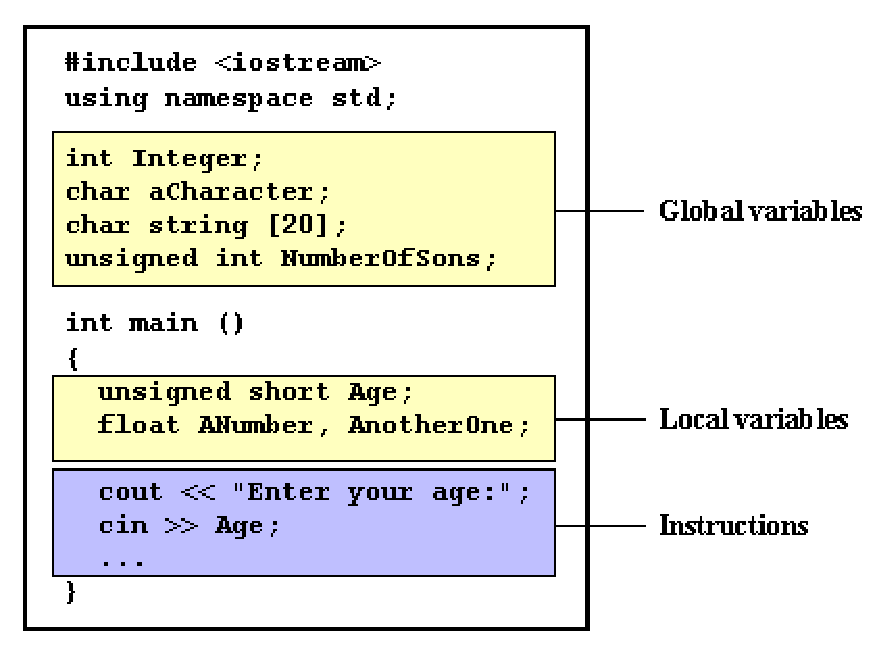
\includegraphics[height=40mm]{./figs/variable_scope.eps}
				\caption{Variable scope\footnotemark.}
			\end{figure}
	  \end{column}
	\end{columns}
	\footnotetext{Source: \url{http://www.cplusplus.com/doc/tutorial/variables/}.}
	\pause
  \dontblock{Declare variables in global scope.  Limit the scope as much as possible to reduce chance of side-effects.  Global constants, however, are fine.}
	

\end{frame}

\section{Operators}

\begin{frame}[fragile]
 \frametitle{Simple operators}
 \begin{block}{Assignment: \texttt{=}}
    \begin{lstlisting}
  a = 5; a = b;
   \end{lstlisting}
  \end{block}
  \pause
  \begin{block}{Arithmetic operators: \texttt{+, -, *, /, \%}}
   All obvious with the exception of the \textit{modulo} operator (\texttt{\%}).  This gives the remainder after division e.g.
  \begin{lstlisting}
  a = 22 % 7;
  \end{lstlisting}
  will set \texttt{a} to \text{1} as $\frac{22}{7} = 3 \times 7 \text{ remainder } 1$.
 \end{block}
 \pause
 \begin{block}{Compound assignment: \texttt{+=, -=, *=, /=, \%=}}
  Perform the operation on the current value of the variable and then set it to the new value, e.g.:
  \begin{lstlisting}
  a += 5; a *= b;
  \end{lstlisting}
 \end{block} %end item
\end{frame}


\begin{frame}[fragile]
  \frametitle{Integer arithmetic}
  
  \begin{warnblocke}
  	In C++ \emph{integer} arithmetic truncates (effectively rounds down):
  	\begin{lstlisting}
  int a = 20;
  int b = 7;
  int someInteger = a / b; // = 2
  	\end{lstlisting}
  	Storing the result in a double doesn't help as the arithmetic has already been done:
  	\begin{lstlisting}
  double someDouble = a / b; // = 2
  double anotherDouble = 20/7; // = 2
  	\end{lstlisting}
  \end{warnblocke}
  	What gives?\\
  	\pause{}  To get around we can ``cast'' the variable to another type:
  	\begin{enumerate}
  	  \item{
  	  	\begin{lstlisting}
someDouble = static_cast<double>(dividend) /
  static_cast<double>(divisor); // = 2.85714
  	  	\end{lstlisting}}
  	  \item{
  	  	\begin{lstlisting}
anotherDouble = 20./7.; // = 2.85714
  	  	\end{lstlisting}}
  	  
  	\end{enumerate}

\end{frame}

\begin{frame}[fragile]
  \begin{block}{Unary operators: \texttt{++, --}}
    \begin{lstlisting}
  a++;
   \end{lstlisting}
   This is equivalent to:
   \begin{lstlisting}
  a += 1;
   \end{lstlisting}
  \end{block}
  \pause
  \begin{block}{Relational and equality operators: \texttt{==, !=, >, <, >=, <=}}
  Evaluates to a boolean (true or false) value e.g.:
    \begin{lstlisting}
  bool areNotEqual = (a != b);
   \end{lstlisting}
 \end{block}
 \pause
 \begin{dontblocke}%
 Mix up \texttt{=} and \texttt{==} this will cause endless headaches!  Consider:
 \begin{lstlisting}
  a = 5; b = 6; areEqual = (a = b);
 \end{lstlisting}
 This is a problem because C++ considers any number other than 0 be true!
 \end{dontblocke}
\end{frame}

\begin{frame}[fragile]
  \begin{block}{Logical operators: \texttt{!, \&\&, ||}}
    These act on boolean values in the following ways:
    \begin{columns}[t]
      \begin{column}[T]{0.2\linewidth}
        NOT
        \begin{tabular}{c|c}
          a & !a \\
          \hline
          \kw{true} & \kw{false} \\
          \kw{false} & \kw{true}
        \end{tabular}
		  \end{column}
		  \begin{column}[T]{0.3\linewidth}
		    AND
		    \begin{tabular}{c|c|c}
		    a & b & a \texttt{\&\&} b \\
		    \hline
		    \kw{true} & \kw{true} & \kw{true} \\
		    \kw{true} & \kw{false} & \kw{false} \\
		    \kw{false} & \kw{true} & \kw{false} \\
		    \kw{false} & \kw{false} & \kw{false}
		    \end{tabular}
      \end{column}
		  \begin{column}[T]{0.3\linewidth}
		    OR
		    \begin{tabular}{c|c|c}		
		    a & b & a \texttt{||} b \\
		    \hline
		    \kw{true} & \kw{true} & \kw{true} \\
		    \kw{true} & \kw{false} & \kw{true} \\
		    \kw{false} & \kw{true} & \kw{true} \\
		    \kw{false} & \kw{false} & \kw{false}
		    \end{tabular}
      \end{column}
    \end{columns}
  \end{block}
  \pause
  \begin{doblocke}
  Keep it simple: don't try and do too much in a single line.  While this:
  \begin{lstlisting}
    result = (i < 10) && (++i < n);
  \end{lstlisting}
  is a valid expression, deciphering what it does is a lot of work.  Instead use:%
  \begin{lstlisting}
    result = i < 10;
    ++i;
    result = result && i < n;
  \end{lstlisting}
%TODO: Check above is true
  \end{doblocke}
\end{frame}

\begin{frame}[fragile]
  \frametitle{Operator precedence}
  \framesubtitle{No, you got first...}
  \begin{columns}[t]
	  \begin{column}[T]{0.44\textwidth}
		  \begin{tabular}{c|l|m{2.1cm}}
			  Precedence & Op. & Associativity \\
			  \hline
			  \multirow{2}{*}{1} & \texttt{++ --} & \multirow{2}{*}{Left to Right}\\
			    & \texttt{!} \\
			  \hline
			  2 & \texttt{* / \%} & \multirow{6}{*}{Left to Right} \\
			  \cline{1-2}
			  3 & \texttt{+ -} & \\
			  \cline{1-2}
			  \multirow{2}{*}{4} & \texttt{< <=} \\
			    & \texttt{> >=} \\
			  \cline{1-2}
			  5 & \texttt{== !=} \\
			  \cline{1-2}
			  6 & \texttt{\&\&} \\
			  \cline{1-2}
			  7 & \texttt{||} \\
			  \hline
			  8 & \texttt{=} & Right to Left
		  \end{tabular}
	 	\end{column}
  	\begin{column}[T]{0.38\textwidth}
	  Operator precedence tells you the order that an expression will be evaluated in.  Some are obvious but consider:
	  \begin{lstlisting}
  a = 21 + 7 % 2;
	  \end{lstlisting}
    which could be interpreted as
	  \begin{lstlisting}
  a = 21 + (7 % 2); // this
  a = (21 + 7) % 2; // or this.
	  \end{lstlisting}
	  In fact the first version is correct.
	  
  	\end{column}
 	\end{columns}
\end{frame}
\begin{frame}
	\doblock{Use parentheses to make an expressions more clear even if they are not necessary.}
\end{frame}

\begin{frame}[fragile]
  \frametitle{Operator precedence}
  \framesubtitle{No, you got first...}
  \begin{columns}[t]
	  \begin{column}[T]{0.44\textwidth}
		  \begin{tabular}{c|l|m{2.1cm}}
			  Precedence & Op. & Associativity \\
			  \hline
			  \multirow{2}{*}{1} & \texttt{++ --} & \multirow{2}{*}{Left to Right}\\
			    & \texttt{!} \\
			  \hline
			  2 & \texttt{* / \%} & \multirow{6}{*}{Left to Right} \\
			  \cline{1-2}
			  3 & \texttt{+ -} & \\
			  \cline{1-2}
			  \multirow{2}{*}{4} & \texttt{< <=} \\
			    & \texttt{> >=} \\
			  \cline{1-2}
			  5 & \texttt{== !=} \\
			  \cline{1-2}
			  6 & \texttt{\&\&} \\
			  \cline{1-2}
			  7 & \texttt{||} \\
			  \hline
			  8 & \texttt{=} & Right to Left
		  \end{tabular}
	 	\end{column}
	  \begin{column}[T]{0.38\textwidth}
	     Operators that have the same precedence are evaluated according to their \textit{associativity} e.g.:
	    \begin{lstlisting}
	a = b = c;   // evaluates as
	a = (b = c);
	    \end{lstlisting}
			because \texttt{=} is right to left associative. 
			\pause  While:
	    \begin{lstlisting}
	a * b % c;
	//evaluates as
	(a * b) % c;
	    \end{lstlisting}
	 are left to right associative. 
	    
	  \end{column}
	\end{columns}
\end{frame}


\section{Basic input and output}

\begin{frame}[fragile]
  \frametitle{Standard output (\texttt{cout})}
  
  You've already met \texttt{cout}, it uses the \textit{indirection operator} (\texttt{<<}) to print to the screen e.g.:
  \begin{lstlisting}
std::cout << "Have some pi: ";
std::cout << 3.1415926;
std::cout << a;
  \end{lstlisting}
  \pause
  We can use \texttt{<<} more than once in the same statement:
  \begin{lstlisting}
double t0 = 1.5, t1 = 2.5;
cout << "t0: " << t0 << ", t1: " << t1
     << ", delta: " << t1 - t0;
  \end{lstlisting}
	\cout{t0: 1.5, t1: 2.5, delta: 1}
	\newline\pause
  If you want a new line you have to use \texttt{\char`\\ n}:
  \begin{lstlisting}
double t0 = 1.5, t1 = 2.5;
cout << "t0: " << t0 << "\nt1: " << t1 << "\n";
  \end{lstlisting}
  \cout{t0: 1.5 \newline t1: 2.5}
% TODO: Change output so it looks alright!
\end{frame}

\begin{frame}[fragile]
  \frametitle{Standard input (\texttt{cin})}
  \framesubtitle{Extracting information out of the user}
  To get input from the user, use the extraction operator (\texttt{>>}) of the \texttt{cin} object (pronounced \textit{see-in}) e.g.:
  \begin{lstlisting}
  double radius;
  std::cin >> radius;
  \end{lstlisting}
  at this point the program will stop and wait for the user to enter a number and push RETURN.
  \pause
  As with output we can use \texttt{>>} more than once in a statement e.g.:
  \begin{lstlisting}
  std::cin >> width >> height;
  \end{lstlisting}
  in this case the program will wait for two sets of numbers to be entered.  They can be separated by a space, tab or a newline.
\end{frame}

\begin{frame}[fragile]
  \frametitle{Complete example}
  \framesubtitle{Putting it all together}
  \lstinputlisting[language=C++,title=\lstsrctitle]{../code/0_basics/lectures/rect_info.cpp}
\end{frame}


\end{document}